\section{Perifer interaktion}
\label{PeriferInteratkion}
%
Igennem følgende afsnit vil forskellige aspekter vedrørende perifer interaktion introduceres, heriblandt to grundprincipper, som perifer interaktion udspringer fra: \textit{Calm Technology} og \textit{Casual Interaction}. Derudover vil potentialet for perifer interaktion undersøges.\blankline
%
Perifer interaktion er ikke nyt. Vi gør det alle sammen, når vi i løbet af vores dagligdag foretager adskillige aktiviteter i vores perifere opmærksomhed, \parencite[s. 1]{PDF:PIIntroduction}. Det forudsætter dog, at disse perifere interaktioner primært retter sig mod ikke-computer-relateret aktiviteter, såsom at føre en samtale imedens der laves mad. Rettes fokus derimod til \textit{Human-Computer-Interaction}, HCI, så forlanger diverse elektroniske apparater vores centrale opmærksomhed ved at blinke, ringe og vibrere, \parencite[s. 1]{PDF:PIIntroduction}. Ifølge \textcite[s. 3]{PDF:PIIntroduction} så bevæger interaktionen med elektroniske apparater sig uforudsigeligt mellem den centrale og perifere opmærksomhed, i modsætning til ikke-computer-relateret aktiviteter, som i større grad kan kontrolleres. Grunden til at disse apparater frit kan bevæge sig fra den perifere til den centrale opmærksomhed skyldes, at vi sjældent har kontrol over hvornår et apparat kræver den centrale opmærksomhed. Så snart et elektronisk apparat befinder sig i den centrale opmærksomhed, så vil ens opmærksomhed midlertidigt fjernes fra den primære opgave, indtil interaktionen med apparatet er afsluttet. Konsekvenserne af at blive forstyrret, og dermed rette sin opmærksomhed væk fra den primære opgave til apparatet, er en øget kognitiv belastning samt en større risiko for at begå fejl i den primære opgave, \parencite[ss. 188-189][s. 162]{PDF:PIDesktopComputingKap9, PDF:ComparingInputModalities}. 

Istedet for at designe elektroniske apparater, som både kræver den centrale opmærksomhed og kræver at opmærksomheden fjernes fra den primære opgave, så bør apparaterne derimod designes, så de i højere grad bliver en integreret del af vores daglige rutiner, \parencite[s. 239]{PDF:PICharacteristicsAndConsiderations}. Ved at designe apparater ud fra den tilgang, vil det tillade perifer interaktion, fordi det, blandt andet, bygger på teori omkring delt-opmærksomhed. Ifølge disse teorier råder mennesket over en bestemt mængde af mentale resourcer, som, afhængigt af opgavernes sværhedsgrad, frit kan distribueres mellem opgaverne, \parencite[s. 240]{PDF:PICharacteristicsAndConsiderations}. Derudover tillader delt-opmærksomhed også, at flere aktiviteter kan foretages samtidigt, så længe de kun kræver få mentale ressourcer, \parencite[s. 2]{PDF:FacilitatingPIDesignAndEvaluation}. Så istedet for at elektroniske apparater kræver den fulde opmærksomhed, så er det ved perifer interaktion muligt at distribuere sin opmærksomhed, for på den måde at foretage flere aktiviter samtidig. Hvis interaktion med computere og andre elektroniske apparater allokeres til den perifere opmærksomhed, kan det ifølge \textcite[s. 11]{PDF:TheComputerWeiser} potentielt fremme det sociale samvær, eksempelvis på arbejdsmarkedet. Derudover pointerer \textcite[s. 11]{PDF:TheComputerWeiser}, at de elektroniske apparater skal tilpasses den menneskelige hverdag og ikke omvendt. Ligeledes bør der tages højde for, at desto flere elektroniske apparater, der produceres til at fange vores centrale opmærksomhed, desto større er behovet for at en del af interaktionen bliver perifer, \parencite[s. 240]{PDF:PICharacteristicsAndConsiderations}.
%
\subsection{Calm Technology og Casual Interaction}
\label{CasualOgCalm}
%
Behovet for at designe elektroniske apparater, som tillader perifer interaktion er ikke nyt. Allerede i halvfemserne blev der af \textcite[s. 3]{PDF:TheComingAgeOfCalmTech} efterspurgt, at såfremt apparaterne skal være allevegne, så skal de ikke være i vejen. I den forbindelse blev \textit{Calm Technology} defineret. Principperne bag \textit{Calm Technology} er simple; ved at allokere noget af interaktionen til den perifere opmærksomhed, er det muligt at håndtere flere informationer ad gangen. Derudover vil allokeringen give en følelse af kontrol, fordi det er muligt selv at kontrollere, hvornår noget er i den centrale kontra den perifere opmærksomhed, \parencite[s. 4]{PDF:TheComingAgeOfCalmTech}. 

\textit{Casual Interaction} er et andet relevant princip, som vedrører hvor meget kontrol der overdrages til et elektronisk apparat, \parencite[ss. 118-119]{PDF:PICasualInteractionKap6}. Med \textit{Casual Interaction} er det muligt at designe apparater, der kan interageres med over en større afstand, som kræver færre kognitive resourcer, som kan interageres med ved hjælp af andre objektet og som kan interageres med uden stor præcision, \parencite[s. 128]{PDF:PICasualInteractionKap6}        
%
\begin{figure}[H]
	\centering
	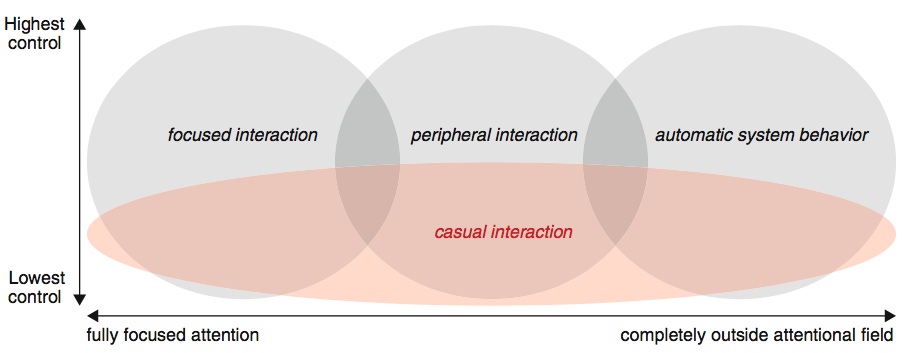
\includegraphics[resolution=300,width=\textwidth]{LevelsOfInteraction}
	\caption{Sammenhæng mellem de tre niveauer af interaktion; fokuseret, perifert og automatisk og hvilket niveau af kontrol, der ønskes samt mængden af opmærksomhed, \parencite[s. 118]{PDF:PICasualInteractionKap6}.}
	\label{fig:LevelsOfInteraction}
\end{figure}
\noindent
%
Det er ved de tre interaktionsniveauer muligt at overdrage kontrol til et elektronisk apparat, hvormed interaktionen bliver afslappet, jævnfør \autoref{fig:LevelsOfInteraction}. Størstedelen af de elektroniske apparater er designet ud fra at interaktionen skal foregå i den centrale opmærksomhed og tilmed kræver fuld kontrol, \parencite[s. 118]{PDF:PICasualInteractionKap6}. Men hvad så, når vi ender i situationer, hvor vi ikke er i stand til eller magter at have den fulde kontrol? Ifølge \textcite[s. 123]{PDF:PICasualInteractionKap6} er der tre årsager til, at vi er villige til at overdrage kontrol til elektroniske apparater; 1) mentale årsager, 2) fysiske årsager og 3) sociale årsager. Et andet spørgsmål, som \textcite[s. 124]{PDF:PICasualInteractionKap6} stiller, vedrører om vi overhovedet er villige til at overdrage kontrol til de elektroniske apparater? Svaret er, at så længe opgaven er tilstrækkeligt let og vi stadig har tilstrækkeligt kontrol til at løse opgaven, så ja, så er vi villige til at overdrage kontrol, \parencite[s. 124]{PDF:PICasualInteractionKap6}.\blankline
%
Ifølge \textcite[s. 6]{PDF:PIIntroduction} udnyttes perifer interaktion ikke i lige så høj grad, som både fokuseret og automatisk interaktion. Til gengæld bliver der i større grad udviklet elektroniske apparater, der understøtter automatisk interaktion, som eksempelvis bevægelsessensorer, der automatisk tænder lyset i et rum så snart der registreres en bevægelse, uanset om hensigten er at tænde lyset, \parencite[s. 5]{PDF:PIIntroduction}.
% 
\subsection{Potentiale for perifer interaktion}
\label{Potentiale}
%
Det tyder kraftigt på, at der findes et uudnyttet område, som har et stort potentiale, hvor det er muligt at designe elektroniske apparater, som aflaster de kognitive resourcer, ikke kræver den centrale opmærksomhed, tillader tilstrækkeligt med kontrol og som potentielt kan fremme vores sociale kompetencer. Det er ihvertfald højst relevant, \parencite[s. 239]{PDF:PICharacteristicsAndConsiderations}, og nødvendigt, \parencite[s. 3]{PDF:TheComingAgeOfCalmTech}, at inddrage og udnytte mulighederne med perifer interaktion i fremtidige elektroniske apparater. 

En af udfordringerne ved at designe et elektronisk apparat, som tillader perifer interaktion er, at apparatet bør være fuldt funktionelt, så det kan testes i den tiltænkte kontekst, \parencite[s. 21]{PDF:EvaluatingPI}. Det skyldes, ifølge \textcite[s. 22]{PDF:EvaluatingPI}, en kombination af at interaktionen først bliver perifer såfremt den er blevet en rutine og af at det er nødvendigt, at apparatet bliver en integreret del af ens hverdag, hvilket er vanskeligt at efterligne i et laboratorium. Så snart en interaktion er blevet en rutine, så vil det medføre at interaktionen kan udføres kun ved hjælp af få mentale ressourcer, hvilket tillader at interaktionen kan foregå i den perifere opmærksomhed, \parencite[s. 2]{PDF:FacilitatingPIDesignAndEvaluation}. Ifølge \textcite[s. 14]{PDF:PIUnseenKap2} så vil interaktionen forblive i det perifere, lige indtil der opstår et problem, som ikke kan løses i den perifere opmærksomhed, hvorfor det flyttes til den centrale opmærksomhed. For at en interaktion kan blive en rutine, bør der tages højde for det menneskelige aspekt, da det formegentligt kan variere fra person til person, hvor svær den givne interaktion er at udføre, \parencite[s. 248]{PDF:PICharacteristicsAndConsiderations}. Selv hvis personen opfatter interaktionen som værende let, så skal de stadig lære at gøre brug af den perifere interaktion frem for den fokuseret interaktion, som de er vant til. Det skyldes, at når og hvis perifer interaktion implementeres, så vil den formegentligt i et eller andet omfang erstatte en i forvejen indlært interaktion, som derfor skal aflæres, \parencite[s. 248]{PDF:PICharacteristicsAndConsiderations}. Denne tilvænningsperiode vil dels afhænge af personens evne til at udføre og indlære den perifere interaktion og dels af, hvor ofte personen har brug for at udføre den. Et godt eksempel på hvornår en interaktion bliver en rutine, og derfor kan foregå i den perifere opmærksomhed, er ved bilkørelse. Det at køre en bil kan, af de fleste, anses som værende en relativ let opgave, men det skyldes udelukkende, at bilister lærer at køre samtidig med, at de tjekker sidespejle, bremser, øger og sænker farten, skifter gear, aktiverer vinduesviskere og slår blinklys til, hvorfor disse interaktioner kan foregå i den perifere opmærksomhed. Hvis det ikke er tilfældet, så er det at køre bil en relativt krævende fysisk såvel som kognitiv opgave. \blankline 
%
Derudover bør det overvejes, hvor perifer interaktion implementeres for bedst muligt at udnytte området mellem fokuseret og automatisk interaktion. På nuværende tidspunkt tyder det på, at perifer interaktion bedst egner sig til små sideopgaver eller understøttende opgaver, \parencite[s. 21]{PDF:EvaluatingPI}. En sideopgave kan eksempelvis være at ændre ens tilgængelighedsstatus på de sociale medier. Sideopgaverne har derfor ikke en direkte forbindelse til den primære opgave, \parencite[s. 162]{PDF:ComparingInputModalities}, hvorimod de understøttende opgaver retter sig mod opgaver, som har en forbindelse til den primære opgave, \parencite[s. 21]{PDF:EvaluatingPI}. Selvom sideopgaverne ikke nødvendigvis er hverken mentalt eller tidsmæssigt krævende, så vil de forårsage dels, at opmærksomheden på den primære opgave fjernes og dels medføre, at der går noget tid før den primære opgave kan genoptages, \parencite[s. 162]{PDF:ComparingInputModalities}. En af årsageren til at sideopgaverne kan virke forstyrrende, skyldes formegentligt at de, ligesom den primære opgave, kræver den visuelle opmærksomhed. Hvis det er tilfældet, så er det ikke muligt at udføre begge opgaver samtidig, hvorfor den ene opgave må vente til den anden er løst, hvilket referer til flaskehalseffekten, \parencite[s. 240]{PDF:PICharacteristicsAndConsiderations}. En måde at udbedre dette problem på kan, blandt andet, være, at designe perifere visuelle displays, som tillader at brugeren bliver bevidst om informationen, uden det forårsager at opmærksomheden fra den primære opgave fjernes, \parencite[s. 247]{PDF:AToolkitForManaging}. Ved at allokere informationen, som de elektroniske apparater giver, så vil det, ifølge \textcite[s. 55]{PDF:PITheoriesKap3}, lede til en bedre brugeroplevelse fordi brugeren ikke overbebyrdes med information, som ikke er relevant for den primære opgave. 

Det tyder på, at hvis udførelsen af sideopgaverne ikke længere befinder sig i den centrale opmærksomhed, men derimod i den perifere opmærksomhed, så vil det have en gavnlig effekt på den primære opgave. Ydermere tyder det på, at det kan være en fordel at overveje, om interaktionen med de elektroniske apparater kan foregå helt eller delvist uden den visuelle opmærksomhed er involveret. Fokus for projektet vil fremadrettet være på én specifik sideopgave, som ikke har en direkte forbindelse til den primære opgave. Derudover tilstræbes det, at interaktionen, som foregår i sideopgaven, ikke vil afhænge af den visuelle opmærksomhed for på den måde at undgå flaskehalseffekten. Ydermere tilstræbes det ligeledes ikke at anvende stemmestyring, da det, ifølge \textcite[s. 41]{PDF:PIEmbeddingHCIMicroManageMe}, er for krævende og dermed ikke kan foregå i den perifere opmærksomhed. Det tyder ydermere på, at det er mindre pinligt, at udføre gestikker i forhold til både stemmestyring og lydkontrol, \parencite[s. 4]{PDF:AnExploratoryStudy}. Der er derfor belæg for ikke at anvende stemmestyring til interaktion med et musikanlæg.

Det kan dog være en fordel at udnytte de motoriske egenskaber, da de, ifølge \textcite[s. 187]{PDF:PIDesktopComputingKap9}, bliver forsømt i HCI. Det skyldes, at interaktionen med computere primært afhænger af ens kognitive egenskaber til at lære og huske forskellige kommandoer, \parencite[s. 187]{PDF:PIDesktopComputingKap9}. Blandt de motoriske egenskaber indgår den proprioceptive sans, som er evnen til opfatte, hvor de enkelte kropsdele er i rummet samt hvordan de er placeret, \parencite[s. 193]{PDF:PIDesktopComputingKap9}. Herunder indgår den kinæstetisk hukommelse, også kaldt muskelhukommelse, som er evnen til at huske en specifik motorisk opgave ved repetition, \parencite[s. 193]{PDF:PIDesktopComputingKap9}. Ved at udnyttet kinæstetisk hukommelse, er det muligt indlære specifikke motoriske opgaver, som efter repetition kræver færre mentale resourcer, hvorfor de kan udføres automatisk og på samme tid som andre opgaver, der ikke kræver aktivering af de samme muskler. Ved at udnytte den proprioceptive sans bør det være muligt at designe elektroniske apparater, som på den måde kan interageres med perifert, hvilket \textcite[s. 202]{PDF:PIDesktopComputingKap9} ligeledes opfordre til.\blankline
%
Da der er afgrænset til at fokusere på én sideløbende opgave; interaktion med et musikanlæg, som ikke har en forbindelse til den primære opgave, samt udnyttelsen af den proprioceptive sans er det oplagt at undersøge hvordan og hvilke typer gestikker, der kan indgå i perifer interaktion og i den forbindelse, hvordan andre har gjort i relaterede undersøgelser.      
 